\chapter{Domain analysis}

\section{Analysis of the party domain}

One of the domains that comes with the negotiation simulator is the \emph{party domain}.
The party domain contains six discrete issues.
These issues and their possible values are:
\begin{itemize}
\item \textbf{Food}: Chips and nuts, finger-food, handmade food, or catering.
\item \textbf{Drinks}: Non-alcoholic, beer only, handmade cocktails, or catering.
\item \textbf{Location}: Party tent, your dorm, party room, or ballroom.
\item \textbf{Invitations}: Plain, photo, custom, handmade, custom, or printed.
\item \textbf{Music}: MP3, DJ, or band.
\item \textbf{Cleanup}: Water and soap, specialized materials, special equipment, or hired help.
\end{itemize}
Additionally, a number of preference profiles is included with the party domain.
Each preference profile assigns a weight to each issue and a numerical value to each possible choice within an issue.
During the negotiation, the preference profile will be used to calculate the utility for bids.

Two of the preference profiles will be examined in detail.
These are \texttt{party\_utility\_kh.xml} and \texttt{party\_utility\_cath.xml}.
KH puts a large weight (0.48) on the location of the party, preferring a party room (5), or a ballroom (3) over the other possible locations, which receive a score of 1.
On the other hand, a weight of 0 is placed on the invitations issue, which means that KH is indifferent between the options.

CATH puts the largest weight on cleanup, and prefers a hired help (20) a lot over the other options (1 to 3).
For most of the issues, this profile shows a large preference for some of the options, as is indicated by the large values assigned to these options.

For all combinations of values, the utility for KH and CATH is calculated.
Those combinations for which there is no solution that is better for one player and not worse for any other form the Pareto-optimal frontier.
The optimal frontier for this problem is shown in Figure \ref{fig:pareto}.
\begin{figure}
\centering
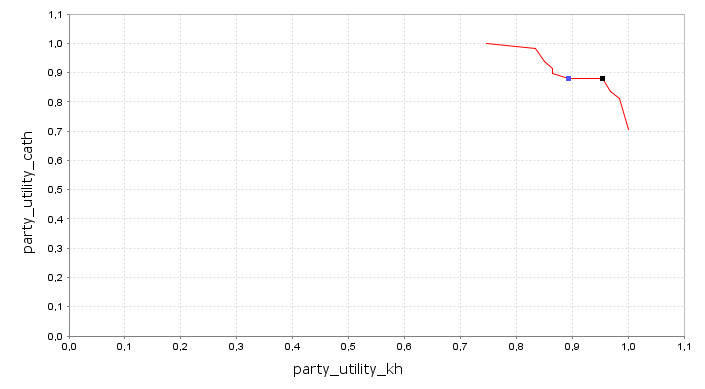
\includegraphics{pareto.png}
\caption{Pareto-optimal frontier for the party domain with preference profiles \texttt{party\_utility\_kh.xml} and \texttt{party\_utility\_cath.xml}. The blue square indicates the position of the Kalai point, the black square represents the Nash point.}
\label{fig:pareto}
\end{figure}


\section{Performance of simple agents}

1b) Analyze the performance of the agent \texttt{SimpleAgent} in the party domain playing against itself. Is a Pareto optimal outcome reached? Explain your answer. Also explain why it obtains the resulting outcome that it does. Do the same for \texttt{Boulware} playing vs. \texttt{Conceder}.